\documentclass[12pt,a4paper,final,leqno]{report}
\usepackage[utf8]{inputenc}
\usepackage[norsk]{babel}
\usepackage{amsmath}
\usepackage{amsfonts}
\usepackage{amssymb}
\usepackage{graphicx}
\usepackage{float}
\usepackage[left=2cm,right=2cm,top=2cm,bottom=2cm]{geometry}
\usepackage{color}
\usepackage{pdfpages}
\sloppy
\definecolor{lightgray}{gray}{0.5}
\setlength{\parindent}{0pt}
\author{Krister Borge }
\title{FYS1120 Oblig2}
\makeindex
\begin{document}
\maketitle

\newpage
\chapter*{Oppgave 2}
\section*{Oppgave 2: Partikkel i magnetisk felt}

I denne oppgaven bruker jeg de den samme partikkelen som i oppgave 1. Euler-Cromers metode for å finne posisjon og fart. Vi bytter ut den det elektriske feltet med et magnetfelt \textbf{B} 
\begin{equation}
\mathbf{F}_B=q(\mathbf{v}\times\mathbf{B})
\end{equation}

\subsection*{Oppgave 2 a)}

Vi bruker samme partikkel. Vi setter $\mathbf{r}(t=0)=(0, 0, 0)$ og $\mathbf{v}(t=0)=(10 km s^{-1}, 0, 0 )$. $\mathbf{B}=(0,0,2T)$
Når vi ser på bevegelsen fra t=0 får jeg disse plottene:

\begin{figure}[H]
\caption{Posisjon}
\centering
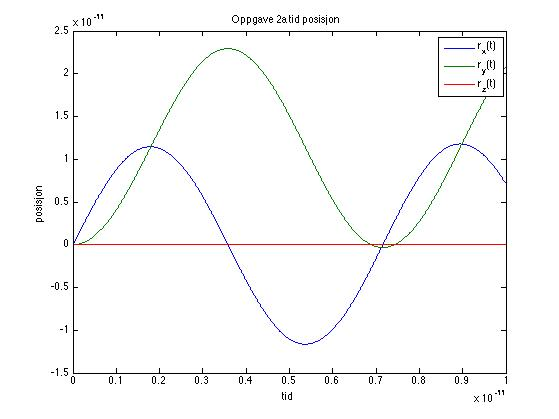
\includegraphics[width=\textwidth]{oppgave2rt.jpg}
\end{figure}

\begin{figure}[H]
\caption{Fart}
\centering
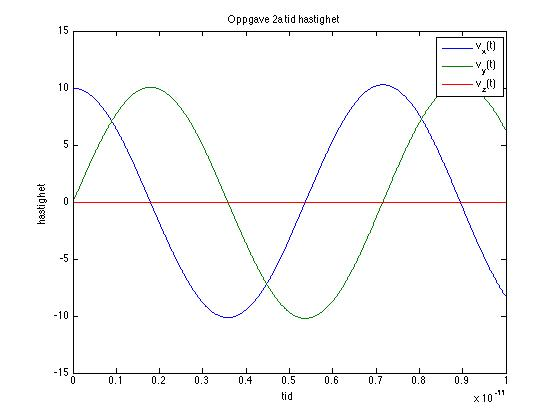
\includegraphics[width=\textwidth]{oppgave2vt.jpg}
\end{figure}

\begin{figure}[H]
\caption{3d}
\centering
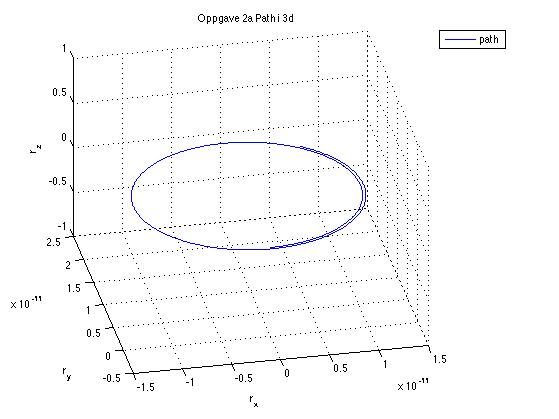
\includegraphics[width=\textwidth]{oppgave23d.jpg}
\end{figure}

\subsection*{Oppgave 2 b)}
Måler omløpstiden T ved å bevege meg langs r. Da blir omløpstiden $1.79\cdot10^{-11}$

\subsection*{Oppgave 2 c)}
 Vis analytisk at syklotronfrekvensen til dette systemet er
 $$
 \omega_c=\frac{q\mathsf{B}}{m}
 $$
 der B=$|\mathbf{B}|$ bruker dette til å vise at
 $$
T=\frac{2\pi m}{q\mathsf{B}}
$$

Jeg vet at F$=ma$ og at v$=\frac{d}{t}$
Skriver F$=m\frac{v^2}{r}$ slik at $qvB=\frac{mv^2}{r}$ og løser for $r$.
$$
qB=\frac{mv}{r}r=>\frac{mv}{qB}
$$
Jeg ser videre på $v=\frac{d}{t}=\frac{2\pi r}{T}$ som gir $T=\frac{2\pi r}{v}$
Setter inn for $r=\frac{mv}{qB} $ og får:
$$
T=\frac{2\pi m}{qB}
$$

\subsection*{Oppgave 2 d)}


\begin{figure}[H]
\caption{Oppgave 2d - Fart}
\centering
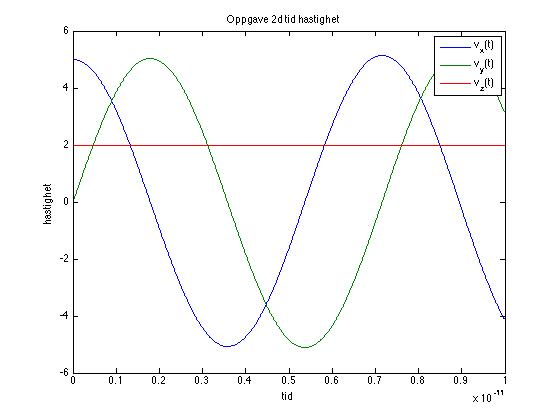
\includegraphics[width=\textwidth]{oppgave2dvt.jpg}
\end{figure}

\begin{figure}[H]
\caption{Oppgave 2 d - 3d}
\centering
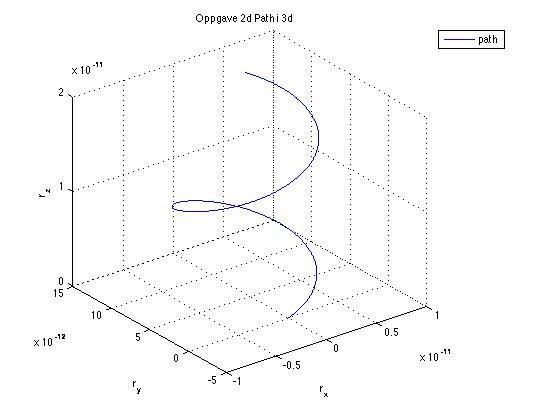
\includegraphics[width=\textwidth]{oppgave2d3d.jpg}
\end{figure}



\chapter*{Oppgave 3 - Partikkel i syklotron}
\subsection*{Oppgave 3 a}
I denne oppgaven ser vi på en partikkels bane i magnetfelt og elektrisk felt.

$$E = \begin{cases} E_0cos(\omega t) \hat{\mathbf{e}}_x, & \mbox{hvis } x \in (d/2, -d/2) \\ (0, 0, 0) & \mbox{ellers}\end{cases}$$

Systemet ser på banen partiklen i feltet. Jeg skal se på bevegelsen til et partikkel i en syklotron med parametere satt tilsvarende den i kjellern på fys.
 

\begin{figure}[H]
\caption{Oppgave 3a -$x_t$ mot $y_t$}
\centering
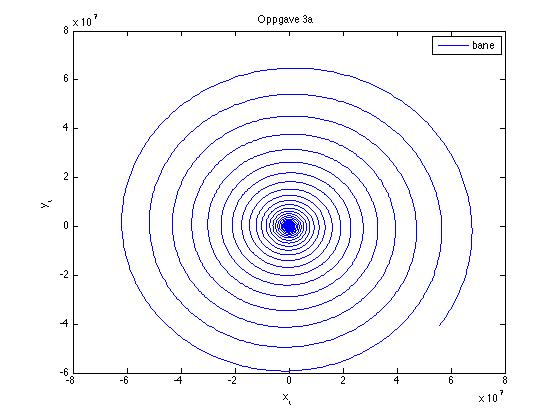
\includegraphics[width=\textwidth]{oppgave3a.jpg}
\end{figure}

Grunnen til at avstanden øker hver runde er at for hver runde i syklotronen vil kraften fra magnetfeltet synke mens akselerasjonen øker. Dette sees tydeligere når man plotter hver x, y og z for seg.
\subsection*{Oppgave 3 b}
Jeg skal implementere at jeg slipper ut et proton ved $r_d$ =50mm. Dette gjør jeg ved å sette grensene for når partiklen er i sirkulasjon i D'ene. 

\begin{figure}[H]
\caption{Posisjon}
\centering
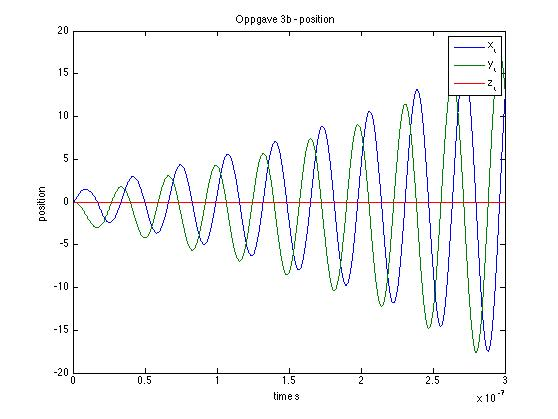
\includegraphics[width=\textwidth]{oppgave3br.jpg}
\end{figure}

\begin{figure}[H]
\caption{fart}
\centering
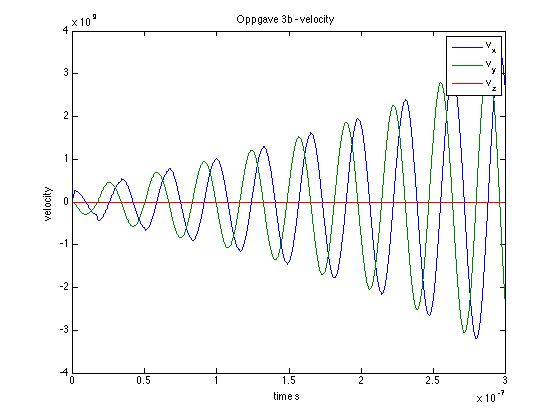
\includegraphics[width=\textwidth]{oppgave3bv.jpg}
\end{figure}

\subsection*{Oppgave 3 c)}

Farten er da: $3.5604\cdot 10^9$
\newpage
\subsection*{Oppgave 3 d)}
Jeg kan vise at den kinetiske enerigen er
$$
E_k=\frac{1}{2}\frac{q^2B^2r^2}{m}
$$
Jeg har at $E_k=\frac{1}{2} mv^2$  jeg vet videre at $v=\frac{qBr}{m}$  og at $r=\frac{mv}{qB}$ 

Setter inn :
$$
E_k=\frac{1}{2} m (\frac{qBr}{m})^2=\frac{1}{2} \frac{q^2B^2r^2}{m}
$$

Jeg regner ut den kinetiske energien i matlab, 
Den kinetiske energien er $E_k = 7.6647 \cdot 10^{-11}$ Joule som tilsvarer 478.3911 MeV.

Hvis jeg ser på massen til protonet (938.272046MeV/c$^2$) og regner ut hvileenergien $E=(938.272046MeV/c^2)*c^2=938.272046MeV$
Sammenlikner jeg hvileenergien til protonet og dens kinetiske energi har jeg at den $E_k$ er 50\% av hvileenergien til protonet.


\chapter*{Oppgave 4 - RC-krets} 
\subsection*{Oppgave 4a)}
\begin{figure}[H]
\caption{ Oppgave aRC-Krets }
\centering
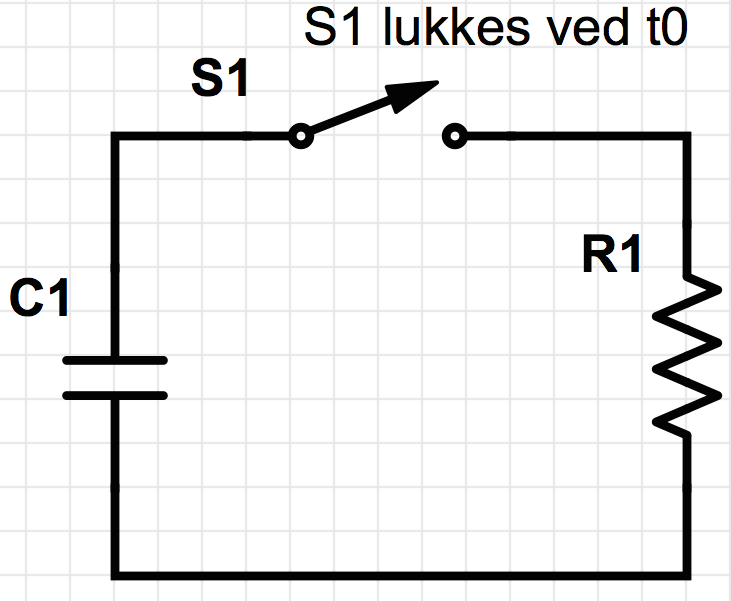
\includegraphics[width=\textwidth]{krets1.jpg}
\end{figure}
\subsection*{Oppgave 4b)}
Her er en krets med en bryter S1, en resistor R og en kondensator C. Ladningen på platene i C er $\pm Q$.

jeg kan finne strømmen i denne kretsen ved å bruke $C=\frac{Q}{V}$, Ohms lov $V=IR$ og definisjonen av strøm $I=\frac{dQ}{dt}$
$$
0=\frac{Q(t)}{C}+I(t)R
$$
$$
I(t)R=-\frac{Q(t)}{C} 
$$
Deler på R og får strømmen I
$$
I(t)=\frac{Q(t)}{RC}=\frac{Q(t)}{\tau}
$$
Definisjonen av strøm gir oss da:
$$
I(t)=\frac{dQ(t)}{dt}=\frac{Q(t)}{\tau}
$$
Ladningen på C faller derfor eksponensielt med tiden:
$$
Q(t)=Q_{max}e^{-\frac{t}{\tau}}
$$
\subsection*{Oppgave 4c}
Strømmen i kretsen er nådd halv parten av $I_max$ ved $0.69 \tau$ siden $e^-0.69\approx 0.5$

\subsection*{Oppgave 4d)}
\begin{figure}[H]
\caption{RC-Krets med batteri med emf $\epsilon$}
\centering
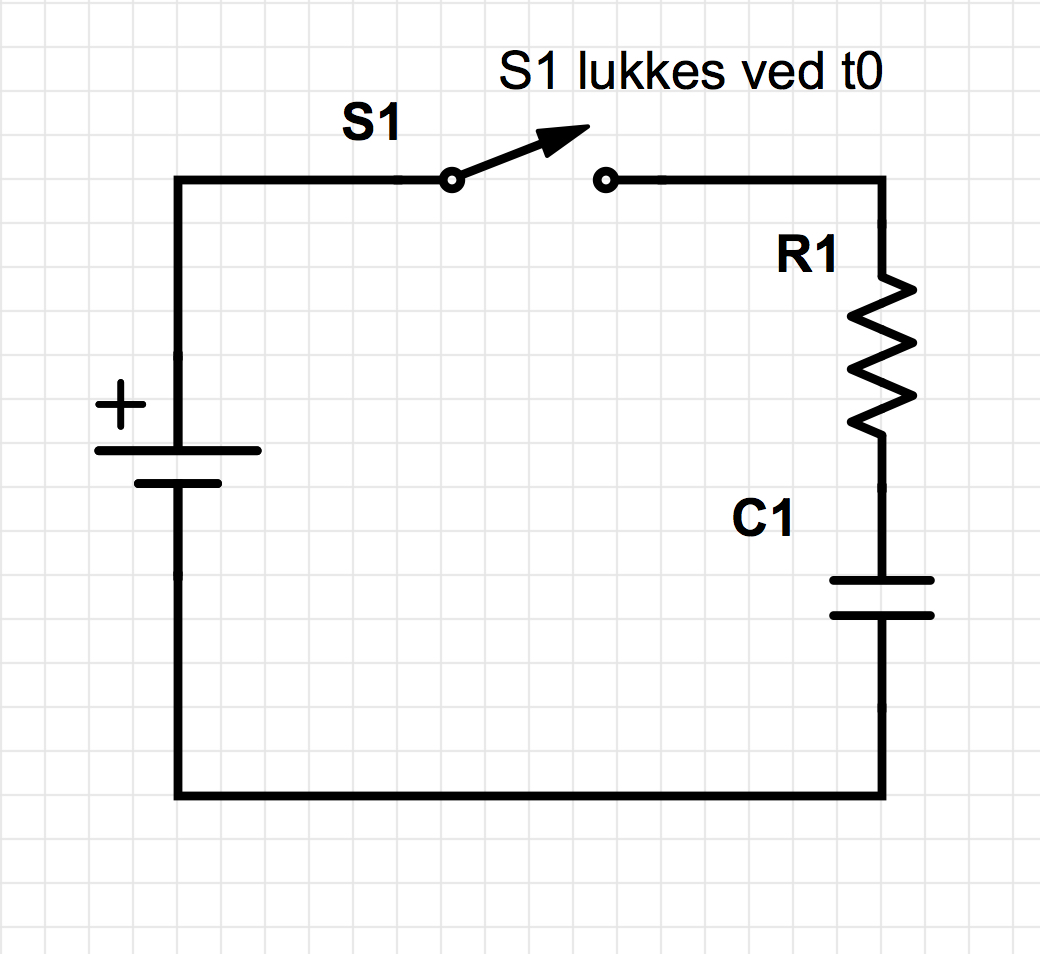
\includegraphics[width=\textwidth]{krets.jpg}
\end{figure}

Nå vil Kirchoff ha noe å si:
$$
\epsilon - V_C-V_R=0
$$
Skriver om 
$$\epsilon - \frac{Q}{C} -Ri=0
$$
$$
\epsilon- \frac{Q}{C}- R \frac{dq}{dt}=0
$$
$$
\frac{dq}{dt}=\frac{1}{RC}(Q-C\epsilon)
$$
$$
\frac{dq}{Q-C\epsilon }=-\frac{dt}{RC}
$$
Integrerer:
$$
\int \frac{dq}{Q-C\epsilon }=-\frac{1}{RC}\int dt
$$
Ladningen er gitt ved:
$$
Q=C\epsilon (1-e^{-t/\tau})
$$
Strømmen blir da:
$$
I=\frac{dQ}{dt}=\frac{\epsilon}{R} e^{-t/\tau}=I_0e^{-t/\tau}
$$
\chapter*{MatLab}
\section{oppgave 3}
\begin{verbatim}

% variabler
m_p = 1.67*10e-27;
e = 1.6*10e-19;
v0 = [0,0,0];
r0 = [0,0,0];
B = [0,0,2]; %B=(0,0,2T)
dt = 1e-10;
t0 = 0;
t1 = 3e-6;
t=t0:dt:t1;
r = r0;
v = v0;
E0 = [90e3/25e-6 0 0 ];
E=E0;
Bs=sqrt(B(:,1)^2 + B(:,2)^2 +B(:,3)^2) ; 
omega = (e*Bs)/m_p;
a=0;
for i=2:length(t)
    
    F_B = e.*(cross(v(i-1,:),B));
    F_E = E.*e;
    F = F_E+F_B;
    
    v(i,:) = v(i-1,:) + a.*dt;
    r(i,:) = r(i-1,:) + v(i-1,:).*dt;
    if (r(i-1,1) <= 0.1 && r(i-1,1) >= -0.1)
        E = E0.*cos(omega*t(i).*[1 0 0]);
   
    else
        E = [0,0,0];
    end
    a = F./m_p;
         
end

figure()
plot(r(:,1), r(:,2))
legend('bane'); title('Oppgave 3a')
xlabel('x_t'); ylabel('y_t')


\end{verbatim}
\begin{verbatim}

m_p = 1.67*10e-27;
e = 1.6*10e-19;
v0 = [0,0,0];
r0 = [0,0,0];
B = [0,0,2]; %B=(0,0,2T)
dt = 100e-12;
t0 = 0;
t1 = 300e-9;
t=t0:dt:t1;
r = r0;
v = v0;
E0 = [90e3/25e-6 0 0 ];
E=E0;
Bs=sqrt(B(:,1)^2 + B(:,2)^2 +B(:,3)^2); 
omega = (e*Bs)/m_p;
r_d = 5e-2;
a=0;
for i=2:length(t)
    
    F_B = e.*(cross(v(i-1,:),B));
    F_E = E.*e;
    F = F_E+F_B;
   
    v(i,:) = v(i-1,:) + a.*dt;
    r(i,:) = r(i-1,:) + v(i-1,:).*dt;
    if (r(i-1,1) <= r_d && r(i-1,1) >= -r_d)
        E = E0.*cos(omega*t(i).*[1 0 0]);
    else
        E = [0,0,0];
    end
    a = F./m_p;
end

figure()
plot(t,r(:,1), t,r(:,2), t, r(:, 3))
legend('x_t','y_t','z_t')
title('Oppgave 3b - position')
xlabel('time s'); ylabel('position')
figure()
plot(t,v(:,1), t,v(:,2), t, v(:, 3))
legend('v_x','v_y','v_z' )
title('Oppgave 3b - velocity')
xlabel('time s'); ylabel('velocity')

fart=sqrt(v(length(v)-1,1)^2+ v(length(v)-1,2)^2+v(length(v)-1,3)^2)
 
\end{verbatim}

\end{document}

